\documentclass{article}\usepackage[]{graphicx}\usepackage[]{color}
% maxwidth is the original width if it is less than linewidth
% otherwise use linewidth (to make sure the graphics do not exceed the margin)
\makeatletter
\def\maxwidth{ %
  \ifdim\Gin@nat@width>\linewidth
    \linewidth
  \else
    \Gin@nat@width
  \fi
}
\makeatother

\definecolor{fgcolor}{rgb}{0.345, 0.345, 0.345}
\newcommand{\hlnum}[1]{\textcolor[rgb]{0.686,0.059,0.569}{#1}}%
\newcommand{\hlstr}[1]{\textcolor[rgb]{0.192,0.494,0.8}{#1}}%
\newcommand{\hlcom}[1]{\textcolor[rgb]{0.678,0.584,0.686}{\textit{#1}}}%
\newcommand{\hlopt}[1]{\textcolor[rgb]{0,0,0}{#1}}%
\newcommand{\hlstd}[1]{\textcolor[rgb]{0.345,0.345,0.345}{#1}}%
\newcommand{\hlkwa}[1]{\textcolor[rgb]{0.161,0.373,0.58}{\textbf{#1}}}%
\newcommand{\hlkwb}[1]{\textcolor[rgb]{0.69,0.353,0.396}{#1}}%
\newcommand{\hlkwc}[1]{\textcolor[rgb]{0.333,0.667,0.333}{#1}}%
\newcommand{\hlkwd}[1]{\textcolor[rgb]{0.737,0.353,0.396}{\textbf{#1}}}%
\let\hlipl\hlkwb

\usepackage{framed}
\makeatletter
\newenvironment{kframe}{%
 \def\at@end@of@kframe{}%
 \ifinner\ifhmode%
  \def\at@end@of@kframe{\end{minipage}}%
  \begin{minipage}{\columnwidth}%
 \fi\fi%
 \def\FrameCommand##1{\hskip\@totalleftmargin \hskip-\fboxsep
 \colorbox{shadecolor}{##1}\hskip-\fboxsep
     % There is no \\@totalrightmargin, so:
     \hskip-\linewidth \hskip-\@totalleftmargin \hskip\columnwidth}%
 \MakeFramed {\advance\hsize-\width
   \@totalleftmargin\z@ \linewidth\hsize
   \@setminipage}}%
 {\par\unskip\endMakeFramed%
 \at@end@of@kframe}
\makeatother

\definecolor{shadecolor}{rgb}{.97, .97, .97}
\definecolor{messagecolor}{rgb}{0, 0, 0}
\definecolor{warningcolor}{rgb}{1, 0, 1}
\definecolor{errorcolor}{rgb}{1, 0, 0}
\newenvironment{knitrout}{}{} % an empty environment to be redefined in TeX

\usepackage{alltt}
\title{Laboratory Assignment 3} 
\author{Katherine Wolf}
\date{\today}

% list of latex packages you'll need
\usepackage{float}  % for tables
\usepackage{mathtools}  % for mathematical symbols
\usepackage{bm}  % to bold mathematical symbols like betas
\usepackage{scrextend}  % to indent subsections
\usepackage{xltxtra,fontspec,xunicode}
\usepackage[dvipsnames]{xcolor}
\usepackage{soul}  % get underlines
\usepackage[skip=0.5\baselineskip]{caption}  % control caption printing space
\usepackage{longtable}

% set fonts
\setmainfont{Georgia}
\setsansfont[Scale=MatchLowercase]{Arial}  % sets the sans font
\setmonofont[Scale=MatchLowercase]{inconsolata}  % sets the monospace font

% make special code formatting
\NewDocumentCommand{\codeword}{v}{%
  \texttt{\textcolor{RoyalPurple}{#1}}%
}

% set the margins of the document
\usepackage[top=1in, bottom=1in, left=.5in, right=.5in]{geometry}
\setlength\parindent{0pt}

% make quick draft versus final versions
\newif\ifdraft  % make draft command
% \draftfalse  % one of these must be commented
\drafttrue  % one of these must be commented

% end the preamble and begin the document
\IfFileExists{upquote.sty}{\usepackage{upquote}}{}
\begin{document}




  \vspace*{-2cm}
  {\let\newpage\relax\maketitle}
  
\maketitle

\ifdraft

\textbf{Read all questions carefully before answering.} You may work in small groups of no more than 3 individuals and turn in a single assignment (and everyone in the group will receive the same grade). Work through the entire assignment individually first, then come together to discuss and collaborate. Please type your responses, \textbf{show your work, and please keep answers brief}.

\section*{Directions}

\vspace{2mm}

Use the dataset \codeword{frmgham_recoded.Rdata} and code provided herein to explore the relationship between smoking status at baseline and time to death in the Framingham cohort.

\begin{knitrout}
\definecolor{shadecolor}{rgb}{0.969, 0.969, 0.969}\color{fgcolor}\begin{kframe}
\begin{alltt}
\hlkwd{load}\hlstd{(}\hlstr{"frmgham_recoded.Rdata"}\hlstd{)}
\hlkwd{library}\hlstd{(survival)}

\hlcom{# create a single-record (retain 1st observation)}
\hlstd{frmgham_recoded} \hlkwb{<-}
  \hlstd{frmgham_recoded[}\hlkwd{which}\hlstd{(frmgham_recoded}\hlopt{$}\hlstd{period} \hlopt{==} \hlnum{1}\hlstd{),]}

\hlcom{# make death into a factor}
\hlstd{frmgham_recoded} \hlkwb{<-}
  \hlstd{frmgham_recoded} \hlopt
  \hlkwd{mutate}\hlstd{(}\hlkwc{death_f} \hlstd{=} \hlkwd{factor}\hlstd{(death))}

\hlcom{# make cursmoke into a factor}
\hlstd{frmgham_recoded} \hlkwb{<-}
  \hlstd{frmgham_recoded} \hlopt
  \hlkwd{mutate}\hlstd{(}\hlkwc{cursmoke_f} \hlstd{=} \hlkwd{factor}\hlstd{(cursmoke))}

\hlcom{# fix sex so that male is 0 and female is 1}
\hlstd{frmgham_recoded} \hlkwb{<-}
  \hlstd{frmgham_recoded} \hlopt
  \hlkwd{mutate}\hlstd{(}\hlkwc{sex_01} \hlstd{= sex} \hlopt{-} \hlnum{1}\hlstd{)}

\hlcom{# fix sex so that male is 0 and female is 1 and a factor}
\hlstd{frmgham_recoded} \hlkwb{<-}
  \hlstd{frmgham_recoded} \hlopt
  \hlkwd{mutate}\hlstd{(}\hlkwc{sex_01_f} \hlstd{=} \hlkwd{factor}\hlstd{(sex} \hlopt{-} \hlnum{1}\hlstd{))}

\hlcom{# make education into a factor}
\hlstd{frmgham_recoded} \hlkwb{<-}
  \hlstd{frmgham_recoded} \hlopt
  \hlkwd{mutate}\hlstd{(}\hlkwc{educ_f} \hlstd{=} \hlkwd{factor}\hlstd{(educ))}
\end{alltt}
\end{kframe}
\end{knitrout}


\vspace{2mm}

The relevant variables for this analysis are:
\begin{itemize}
  \item \codeword{time_yrs} (time of entry into study)
  \item \codeword{death} (indicator of death [=1] or censored [=0])
  \item \codeword{cursmoke} (indicator of current smoking status: yes (1) vs. no (0))
  \item \codeword{age} (age in years)
  \item \codeword{sex} (variable denoting male (1) or female (2); \textbf{use 1 as referent category})
  \item \codeword{educ} (educational status, nominal categories 1-4; \textbf{use 1 as referent category})
\end{itemize}

Adapting the code presented in the lecture, and the additional piece below, complete the following tasks:

\vspace{2mm}

\textbf{Describing survival data (Questions 1-2, part of 7)}

\begin{itemize}
  \item Referring to the code from the lecture notes, \textbf{plot the Kaplan-Meier estimate of the survival function} for each smoking category (using the variable cursmoke) for these data.
  
1. Call in the `survival` package.   
2. Recode `status` so that death = 1 and censored = 0.   
3. Use `Surv()` to set up your outcome object.   
4. Use `survfit` with `conf.type = "log-log"` to estimate the K-M survival function.   
5. Plot the K-M survival curve using `plot(survival\_object, bty = "l")`   
6. Estimate the median survival time using the `quantile` function.   
  
\begin{knitrout}
\definecolor{shadecolor}{rgb}{0.969, 0.969, 0.969}\color{fgcolor}\begin{kframe}
\begin{alltt}
\hlcom{#### make kaplan-meier model}
\hlstd{s_death} \hlkwb{<-}
  \hlkwd{with}\hlstd{(}
    \hlstd{frmgham_recoded,}
    \hlkwd{Surv}\hlstd{(}
      \hlkwc{time} \hlstd{= timedth_yrs,}
      \hlkwc{event} \hlstd{= death)}
    \hlstd{)}

\hlstd{km_death} \hlkwb{<-}
  \hlkwd{with}\hlstd{(}
    \hlstd{frmgham_recoded,}
    \hlkwd{survfit}\hlstd{(}
      \hlstd{s_death} \hlopt{~} \hlnum{1}\hlstd{)}
    \hlstd{)}

\hlstd{km_death_smoke} \hlkwb{<-}
  \hlkwd{with}\hlstd{(}
    \hlstd{frmgham_recoded,}
    \hlkwd{survfit}\hlstd{(}
      \hlstd{s_death} \hlopt{~} \hlstd{cursmoke)}
    \hlstd{)}

\hlkwd{ggsurvplot}\hlstd{(}
  \hlstd{km_death_smoke,}
  \hlkwc{data} \hlstd{= frmgham_recoded,}
  \hlkwc{title} \hlstd{=} \hlstr{"Kaplan-Meier Survival Estimates by Current Smoking Status"}\hlstd{,}
  \hlkwc{xlab} \hlstd{=} \hlstr{"Time (years)"}\hlstd{,}
  \hlkwc{ylab} \hlstd{=} \hlstr{"Survival Probability"}
\hlstd{)}
\end{alltt}
\end{kframe}
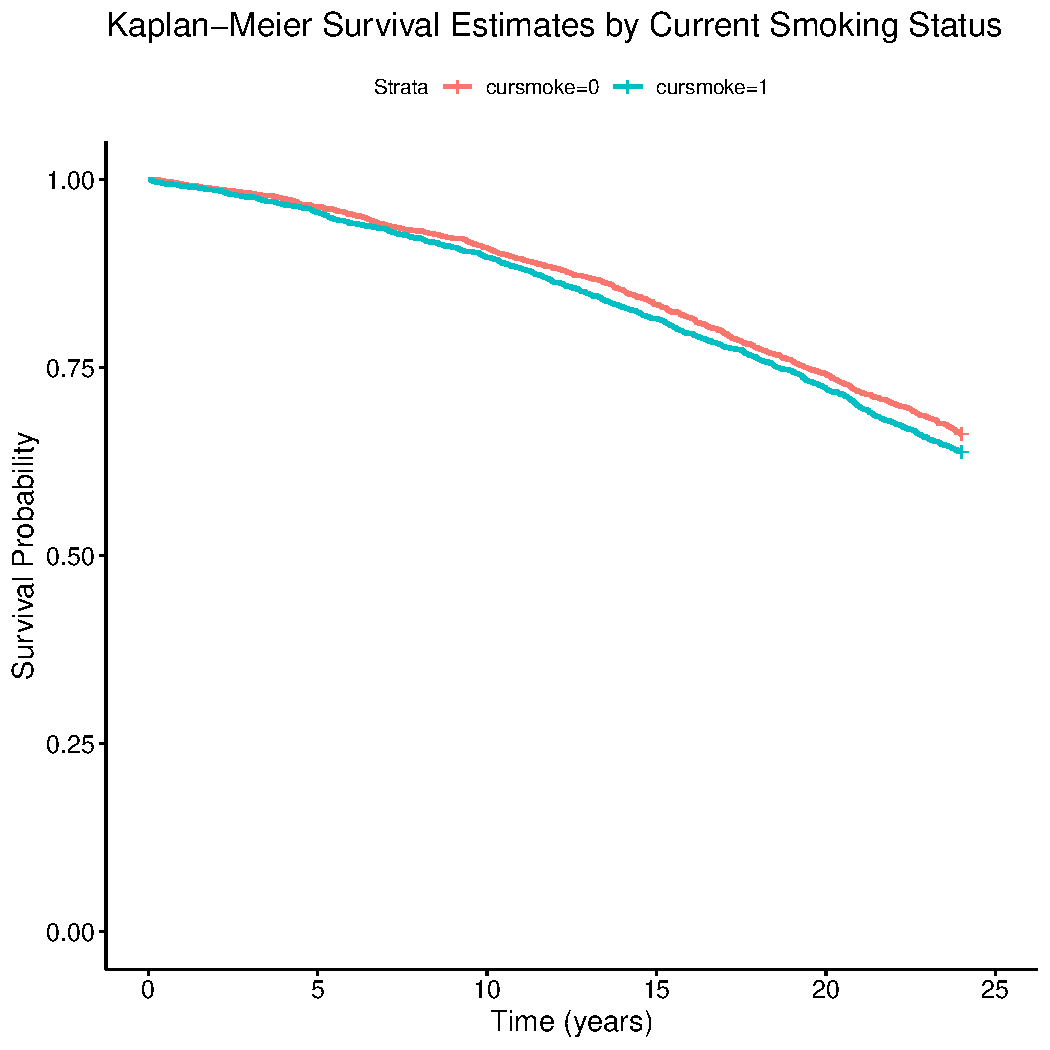
\includegraphics[width=\maxwidth]{figure/unnamed-chunk-3-1} 

\end{knitrout}
  
  \item Using the code below, \textbf{calculate the number of events and number of person-years in each exposure group}:
\end{itemize}


\begin{knitrout}
\definecolor{shadecolor}{rgb}{0.969, 0.969, 0.969}\color{fgcolor}\begin{kframe}
\begin{alltt}
\hlcom{# The "scale" option set to 1 tells pyears() that the time is already in yrs}
\hlcom{# (default is to divide time by 365.25)}
\hlstd{py.smoke} \hlkwb{<-} \hlkwd{pyears}\hlstd{(}\hlkwd{Surv}\hlstd{(timedth_yrs, death)} \hlopt{~} \hlstd{cursmoke_f,}
                   \hlstd{frmgham_recoded,}
                   \hlkwc{scale} \hlstd{=} \hlnum{1}\hlstd{)[}\hlkwd{c}\hlstd{(}\hlstr{"event"}\hlstd{,} \hlstr{"pyears"}\hlstd{)]}

\hlcom{# Make it pretty}
\hlkwd{simplify2array}\hlstd{(py.smoke)}
\end{alltt}
\begin{verbatim}
##           
## cursmoke_f event   pyears
##          0   762 46675.20
##          1   788 44440.38
\end{verbatim}
\end{kframe}
\end{knitrout}


\textbf{Proportional hazards modeling (Questions 3-8)}
\begin{itemize}
  \item Referring to the code from the lecture notes, \textbf{use the log-rank test to determine if there are any differences in survival between the smoking groups}.
  

\begin{knitrout}
\definecolor{shadecolor}{rgb}{0.969, 0.969, 0.969}\color{fgcolor}\begin{kframe}
\begin{alltt}
\hlkwd{survdiff}\hlstd{(s_death} \hlopt{~} \hlstd{cursmoke_f,}
         \hlkwc{data} \hlstd{= frmgham_recoded)}
\end{alltt}
\begin{verbatim}
## Call:
## survdiff(formula = s_death ~ cursmoke_f, data = frmgham_recoded)
## 
##                 N Observed Expected (O-E)^2/E (O-E)^2/V
## cursmoke_f=0 2253      762      796      1.42      2.91
## cursmoke_f=1 2181      788      754      1.49      2.91
## 
##  Chisq= 2.9  on 1 degrees of freedom, p= 0.09
\end{verbatim}
\end{kframe}
\end{knitrout}

  \item \textbf{Using a Cox proportional hazards regression model}, estimate the association between current smoking status (at baseline) and time to death. Estimate 2 models:
  \begin{itemize}
    \item An \textbf{unadjusted} model (only including smoking status), and
    
\begin{knitrout}
\definecolor{shadecolor}{rgb}{0.969, 0.969, 0.969}\color{fgcolor}\begin{kframe}
\begin{alltt}
\hlstd{coxph_death_smoke} \hlkwb{<-}
  \hlkwd{coxph}\hlstd{(s_death} \hlopt{~} \hlstd{cursmoke,} \hlcom{# the regression formula}
                    \hlkwc{data} \hlstd{= frmgham_recoded,} \hlcom{# the data}
                    \hlkwc{ties} \hlstd{=} \hlstr{"efron"}\hlstd{)} \hlcom{# how to handle ties}

\hlkwd{summary}\hlstd{(coxph_death_smoke)} \hlcom{# Model output}
\end{alltt}
\begin{verbatim}
## Call:
## coxph(formula = s_death ~ cursmoke, data = frmgham_recoded, ties = "efron")
## 
##   n= 4434, number of events= 1550 
## 
##             coef exp(coef) se(coef)     z Pr(>|z|)  
## cursmoke 0.08668   1.09055  0.05081 1.706    0.088 .
## ---
## Signif. codes:  0 '***' 0.001 '**' 0.01 '*' 0.05 '.' 0.1 ' ' 1
## 
##          exp(coef) exp(-coef) lower .95 upper .95
## cursmoke     1.091      0.917    0.9872     1.205
## 
## Concordance= 0.511  (se = 0.006 )
## Likelihood ratio test= 2.91  on 1 df,   p=0.09
## Wald test            = 2.91  on 1 df,   p=0.09
## Score (logrank) test = 2.91  on 1 df,   p=0.09
\end{verbatim}
\end{kframe}
\end{knitrout}
    
    \item An \textbf{adjusted} model that also includes age (continuous), sex (binary) and education (4-category) in this model. (For nominal categorical variables, you may need to use the \codeword{factor()} operator in the formula as demonstrated in class.)
    
\begin{knitrout}
\definecolor{shadecolor}{rgb}{0.969, 0.969, 0.969}\color{fgcolor}\begin{kframe}
\begin{alltt}
\hlcom{# fit adjusted model}
\hlstd{coxph_death_smoke_adjusted} \hlkwb{<-}
  \hlkwd{coxph}\hlstd{(s_death} \hlopt{~} \hlstd{cursmoke_f} \hlopt{+} \hlstd{age} \hlopt{+} \hlstd{sex_01_f} \hlopt{+} \hlstd{educ_f,}
        \hlkwc{data} \hlstd{= frmgham_recoded,}
        \hlkwc{ties} \hlstd{=} \hlstr{"efron"}\hlstd{)}

\hlkwd{summary}\hlstd{(coxph_death_smoke_adjusted)}
\end{alltt}
\begin{verbatim}
## Call:
## coxph(formula = s_death ~ cursmoke_f + age + sex_01_f + educ_f, 
##     data = frmgham_recoded, ties = "efron")
## 
##   n= 4321, number of events= 1509 
##    (113 observations deleted due to missingness)
## 
##                  coef exp(coef)  se(coef)       z Pr(>|z|)    
## cursmoke_f1  0.339445  1.404167  0.054351   6.245 4.23e-10 ***
## age          0.095630  1.100351  0.003386  28.240  < 2e-16 ***
## sex_01_f1   -0.549651  0.577151  0.053874 -10.203  < 2e-16 ***
## educ_f2     -0.037740  0.962963  0.064130  -0.588 0.556201    
## educ_f3     -0.167686  0.845619  0.078855  -2.127 0.033460 *  
## educ_f4     -0.324557  0.722847  0.092120  -3.523 0.000426 ***
## ---
## Signif. codes:  0 '***' 0.001 '**' 0.01 '*' 0.05 '.' 0.1 ' ' 1
## 
##             exp(coef) exp(-coef) lower .95 upper .95
## cursmoke_f1    1.4042     0.7122    1.2623    1.5620
## age            1.1004     0.9088    1.0931    1.1077
## sex_01_f1      0.5772     1.7326    0.5193    0.6414
## educ_f2        0.9630     1.0385    0.8492    1.0919
## educ_f3        0.8456     1.1826    0.7245    0.9870
## educ_f4        0.7228     1.3834    0.6034    0.8659
## 
## Concordance= 0.724  (se = 0.006 )
## Likelihood ratio test= 1038  on 6 df,   p=<2e-16
## Wald test            = 979.3  on 6 df,   p=<2e-16
## Score (logrank) test = 1061  on 6 df,   p=<2e-16
\end{verbatim}
\end{kframe}
\end{knitrout}
    
  \end{itemize}
  \item Estimate a model with \textbf{an interaction between linear follow-up time} and \ul{all} of the covariates in the model. \textit{(Hint: you will need to use the ‘tt()‘ function within the ‘coxph‘ command.)}
\end{itemize}

\begin{knitrout}
\definecolor{shadecolor}{rgb}{0.969, 0.969, 0.969}\color{fgcolor}\begin{kframe}
\begin{alltt}
\hlstd{cox_time_death_smoke_factored} \hlkwb{<-}
  \hlkwd{coxph}\hlstd{(}\hlkwd{Surv}\hlstd{(timedth_yrs, death)} \hlopt{~}
          \hlstd{cursmoke_f} \hlopt{+}
          \hlstd{age} \hlopt{+}
          \hlstd{sex_01_f} \hlopt{+}
          \hlstd{educ_f} \hlopt{+}
          \hlkwd{tt}\hlstd{(cursmoke)} \hlopt{+}
          \hlkwd{tt}\hlstd{(age)} \hlopt{+}
          \hlkwd{tt}\hlstd{(sex_01)} \hlopt{+}
          \hlkwd{tt}\hlstd{(}\hlkwd{as.integer}\hlstd{(educ_f} \hlopt{==} \hlnum{2}\hlstd{))} \hlopt{+}
          \hlkwd{tt}\hlstd{(}\hlkwd{as.integer}\hlstd{(educ_f} \hlopt{==} \hlnum{3}\hlstd{))} \hlopt{+}
          \hlkwd{tt}\hlstd{(}\hlkwd{as.integer}\hlstd{(educ_f} \hlopt{==} \hlnum{4}\hlstd{)),}
        \hlkwc{data} \hlstd{= frmgham_recoded,}
        \hlkwc{method} \hlstd{=} \hlstr{"efron"}\hlstd{,}
        \hlkwc{tt} \hlstd{=} \hlkwa{function}\hlstd{(}\hlkwc{x}\hlstd{,}\hlkwc{t}\hlstd{,}\hlkwc{...}\hlstd{) x}\hlopt{*}\hlstd{t)}

\hlkwd{summary}\hlstd{(cox_time_death_smoke_factored)}
\end{alltt}
\begin{verbatim}
## Call:
## coxph(formula = Surv(timedth_yrs, death) ~ cursmoke_f + age + 
##     sex_01_f + educ_f + tt(cursmoke) + tt(age) + tt(sex_01) + 
##     tt(as.integer(educ_f == 2)) + tt(as.integer(educ_f == 3)) + 
##     tt(as.integer(educ_f == 4)), data = frmgham_recoded, tt = function(x, 
##     t, ...) x * t, method = "efron")
## 
##   n= 4321, number of events= 1509 
##    (113 observations deleted due to missingness)
## 
##                                   coef  exp(coef)   se(coef)      z Pr(>|z|)
## cursmoke_f1                  0.4363723  1.5470847  0.1305887  3.342 0.000833
## age                          0.0877577  1.0917235  0.0080509 10.900  < 2e-16
## sex_01_f1                   -0.2903968  0.7479667  0.1293844 -2.244 0.024804
## educ_f2                      0.0024753  1.0024783  0.1541964  0.016 0.987192
## educ_f3                     -0.1723551  0.8416802  0.1933545 -0.891 0.372718
## educ_f4                     -0.2593351  0.7715645  0.2239116 -1.158 0.246781
## tt(cursmoke)                -0.0068349  0.9931884  0.0084028 -0.813 0.415985
## tt(age)                      0.0005738  1.0005740  0.0005211  1.101 0.270795
## tt(sex_01)                  -0.0184881  0.9816817  0.0083232 -2.221 0.026332
## tt(as.integer(educ_f == 2)) -0.0029913  0.9970132  0.0098984 -0.302 0.762499
## tt(as.integer(educ_f == 3))  0.0002182  1.0002182  0.0122545  0.018 0.985795
## tt(as.integer(educ_f == 4)) -0.0048224  0.9951892  0.0141866 -0.340 0.733912
##                                
## cursmoke_f1                 ***
## age                         ***
## sex_01_f1                   *  
## educ_f2                        
## educ_f3                        
## educ_f4                        
## tt(cursmoke)                   
## tt(age)                        
## tt(sex_01)                  *  
## tt(as.integer(educ_f == 2))    
## tt(as.integer(educ_f == 3))    
## tt(as.integer(educ_f == 4))    
## ---
## Signif. codes:  0 '***' 0.001 '**' 0.01 '*' 0.05 '.' 0.1 ' ' 1
## 
##                             exp(coef) exp(-coef) lower .95 upper .95
## cursmoke_f1                    1.5471     0.6464    1.1977    1.9983
## age                            1.0917     0.9160    1.0746    1.1091
## sex_01_f1                      0.7480     1.3370    0.5804    0.9639
## educ_f2                        1.0025     0.9975    0.7410    1.3562
## educ_f3                        0.8417     1.1881    0.5762    1.2295
## educ_f4                        0.7716     1.2961    0.4975    1.1966
## tt(cursmoke)                   0.9932     1.0069    0.9770    1.0097
## tt(age)                        1.0006     0.9994    0.9996    1.0016
## tt(sex_01)                     0.9817     1.0187    0.9658    0.9978
## tt(as.integer(educ_f == 2))    0.9970     1.0030    0.9779    1.0165
## tt(as.integer(educ_f == 3))    1.0002     0.9998    0.9765    1.0245
## tt(as.integer(educ_f == 4))    0.9952     1.0048    0.9679    1.0232
## 
## Concordance= 0.725  (se = 0.006 )
## Likelihood ratio test= 1045  on 12 df,   p=<2e-16
## Wald test            = 987.7  on 12 df,   p=<2e-16
## Score (logrank) test = 1070  on 12 df,   p=<2e-16
\end{verbatim}
\end{kframe}
\end{knitrout}


\begin{knitrout}
\definecolor{shadecolor}{rgb}{0.969, 0.969, 0.969}\color{fgcolor}\begin{kframe}
\begin{alltt}
\hlstd{cox_time_death_smoke_not_factored} \hlkwb{<-}
  \hlkwd{coxph}\hlstd{(}\hlkwd{Surv}\hlstd{(timedth_yrs, death)} \hlopt{~}
          \hlstd{cursmoke} \hlopt{+}
          \hlstd{age} \hlopt{+}
          \hlstd{sex_01} \hlopt{+}
          \hlkwd{factor}\hlstd{(educ)} \hlopt{+}
          \hlkwd{tt}\hlstd{(cursmoke)} \hlopt{+}
          \hlkwd{tt}\hlstd{(age)} \hlopt{+}
          \hlkwd{tt}\hlstd{(sex_01)} \hlopt{+}
          \hlkwd{tt}\hlstd{(}\hlkwd{as.integer}\hlstd{(educ} \hlopt{==} \hlnum{2}\hlstd{))} \hlopt{+}
          \hlkwd{tt}\hlstd{(}\hlkwd{as.integer}\hlstd{(educ} \hlopt{==} \hlnum{3}\hlstd{))} \hlopt{+}
          \hlkwd{tt}\hlstd{(}\hlkwd{as.integer}\hlstd{(educ} \hlopt{==} \hlnum{4}\hlstd{)),}
        \hlkwc{data} \hlstd{= frmgham_recoded,}
        \hlkwc{method} \hlstd{=} \hlstr{"efron"}\hlstd{,}
        \hlkwc{tt} \hlstd{=} \hlkwa{function}\hlstd{(}\hlkwc{x}\hlstd{,}\hlkwc{t}\hlstd{,}\hlkwc{...}\hlstd{) x}\hlopt{*}\hlstd{t)}

\hlkwd{summary}\hlstd{(cox_time_death_smoke_not_factored)}
\end{alltt}
\begin{verbatim}
## Call:
## coxph(formula = Surv(timedth_yrs, death) ~ cursmoke + age + sex_01 + 
##     factor(educ) + tt(cursmoke) + tt(age) + tt(sex_01) + tt(as.integer(educ == 
##     2)) + tt(as.integer(educ == 3)) + tt(as.integer(educ == 4)), 
##     data = frmgham_recoded, tt = function(x, t, ...) x * t, method = "efron")
## 
##   n= 4321, number of events= 1509 
##    (113 observations deleted due to missingness)
## 
##                                 coef  exp(coef)   se(coef)      z Pr(>|z|)    
## cursmoke                   0.4363723  1.5470847  0.1305887  3.342 0.000833 ***
## age                        0.0877577  1.0917235  0.0080509 10.900  < 2e-16 ***
## sex_01                    -0.2903968  0.7479667  0.1293844 -2.244 0.024804 *  
## factor(educ)2              0.0024753  1.0024783  0.1541964  0.016 0.987192    
## factor(educ)3             -0.1723551  0.8416802  0.1933545 -0.891 0.372718    
## factor(educ)4             -0.2593351  0.7715645  0.2239116 -1.158 0.246781    
## tt(cursmoke)              -0.0068349  0.9931884  0.0084028 -0.813 0.415985    
## tt(age)                    0.0005738  1.0005740  0.0005211  1.101 0.270795    
## tt(sex_01)                -0.0184881  0.9816817  0.0083232 -2.221 0.026332 *  
## tt(as.integer(educ == 2)) -0.0029913  0.9970132  0.0098984 -0.302 0.762499    
## tt(as.integer(educ == 3))  0.0002182  1.0002182  0.0122545  0.018 0.985795    
## tt(as.integer(educ == 4)) -0.0048224  0.9951892  0.0141866 -0.340 0.733912    
## ---
## Signif. codes:  0 '***' 0.001 '**' 0.01 '*' 0.05 '.' 0.1 ' ' 1
## 
##                           exp(coef) exp(-coef) lower .95 upper .95
## cursmoke                     1.5471     0.6464    1.1977    1.9983
## age                          1.0917     0.9160    1.0746    1.1091
## sex_01                       0.7480     1.3370    0.5804    0.9639
## factor(educ)2                1.0025     0.9975    0.7410    1.3562
## factor(educ)3                0.8417     1.1881    0.5762    1.2295
## factor(educ)4                0.7716     1.2961    0.4975    1.1966
## tt(cursmoke)                 0.9932     1.0069    0.9770    1.0097
## tt(age)                      1.0006     0.9994    0.9996    1.0016
## tt(sex_01)                   0.9817     1.0187    0.9658    0.9978
## tt(as.integer(educ == 2))    0.9970     1.0030    0.9779    1.0165
## tt(as.integer(educ == 3))    1.0002     0.9998    0.9765    1.0245
## tt(as.integer(educ == 4))    0.9952     1.0048    0.9679    1.0232
## 
## Concordance= 0.725  (se = 0.006 )
## Likelihood ratio test= 1045  on 12 df,   p=<2e-16
## Wald test            = 987.7  on 12 df,   p=<2e-16
## Score (logrank) test = 1070  on 12 df,   p=<2e-16
\end{verbatim}
\end{kframe}
\end{knitrout}

% put only code chunks with "FALSE" here to produce final document

\else

\fi

\section*{Questions}

\vspace{2mm}

\begin{enumerate}
  \item Using the Kaplan-Meier plots, graphically assess the relationship between baseline smoking status and time to death. \textbf{Briefly interpret what you see.} In 1-2 sentences describe the limitations of this approach. [{\ul{include the graph}}, labeled \textbf{Figure 1}] \textbf{(10 points)}
  \item \textbf{Referring to the code from lecture}, are you able to calculate the overall median survival time in this case? If so, provide an estimate of this quantity, if not, describe why and provide an estimate of a percentile of survival time (of your choice). Interpret the quantity that you estimated. \textbf{(20 points)}
  \item Answer the following questions about the log-rank test: \textbf{(10 points total)}
  \begin{enumerate}
    \item Describe the specific null and alternative hypotheses that the log-rank test is considering here.
    \item What do you conclude from this test (use 5\% significance criteria)? List a limitation of the inference that you obtain from the log-rank test.
  \end{enumerate}
\item Answer the following questions about the Cox models estimated above: \textbf{(20 points total)}
  \begin{enumerate}
    \item Why do we use specialized methods for survival analysis (instead of linear or logistic regression, for example)? (Hint: See readings from Vittinghoff et al. 2012 text.)
    \item What are the advantages of the Cox model over other survival analysis methods? What is a potential disadvantage of the Cox model?
    \item What assumptions, if any, does the standard \textbf{Cox} proportional hazards model make?
    \item Compare the test of the smoking-mortality association between the log-rank test and the likelihood ratio test from the \ul{unadjusted} Cox proportional hazards model. What do you observe? Between these two analytic approaches, which one would you prefer, and why?
  \end{enumerate}
  \item Write the equation for the log-hazard function for the \textit{adjusted} model you estimated. \textbf{Clearly define all functions, terms (covariates), and parameters in the model. (20 points)}
  \item Complete the following table. How would you interpret the parameter estimate that compares smokers to non-smokers in the \textbf{adjusted model}? What measure of association common in epidemiologic research does this correspond to? \textbf{(10 points)}




% latex table generated in R 3.6.1 by xtable 1.8-4 package
% Sun Nov 24 00:23:59 2019
\begin{table}[H]
\centering
\parbox{10cm}{\caption{Crude and adjusted hazard ratio (HR) estimates of the association between baseline smoking status and mortality. Framingham Cohort Study. 1948-1972, Framingham, MA.}} 
\begin{tabular}{lllll}
  \hline
Smoker & Events & Follow-Up Time (years) & Crude HR (95\% CI) & Adjusted HR (95\% CI) \\ 
  \hline
No &  &  &  &  \\ 
  Yes &  &  &  &  \\ 
   \hline
\end{tabular}
\end{table}

  
  \item Based on the model that included covariate-by-time interactions, is there evidence for a violation of the proportional hazards assumption in any of the variables? Indicate how you arrived at your conclusion. \ul{In 1-2 sentences} describe in general how you would account for any violations in the proportional hazards assumption (ignoring whether or not there were significant differences here). \textbf{(10 points)}
\end{enumerate}

\pagebreak

\section*{Question 1}

\ifdraft

Using the Kaplan-Meier plots, graphically assess the relationship between baseline smoking status and time to death. \textbf{Briefly interpret what you see.} In 1-2 sentences describe the limitations of this approach. [{\ul{include the graph}}, labeled \textbf{Figure 1}] \textbf{(10 points)}

\fi



Participants who were current smokers at the start of the study appear to have lower probabilities of survival at all time points than participants who were not current smokers at the start of the study, and the gap between the groups appears to widen slightly over the course of the study until its end at 24 years, when the probability of survival for the smokers was 63.87\% and the probability of survival for the nonsmokers was 66.18\%.

\vspace{2mm}

Although Kaplan-Meier estimates of survival curves offer the advantages of 
\begin{itemize}
  \item estimating survival probabilities accurately even in the presence of censored observations during the study period, and
  \item being nonparametric, i.e., making no assumptions about the distribution of survival times in the cohort,
\end{itemize}

major limitations of simple visual comparison of the graphs of the survival curves of the two groups include 

\begin{itemize}
  \item the failure to account or control for the effects of any covariates that might have confounded or mediated the relationship between smoking and survival time, and
  \item the absence of a formal test of the hypothesis that the survival probabilities are systematically different between the groups over the study period (versus to the null hypothesis the apparent difference on the graph between the two curves resulted from chance alone).
  
\end{itemize}

Figure 1. Kaplan-Meier Survival Estimates by Current Smoking Status







\begin{knitrout}
\definecolor{shadecolor}{rgb}{0.969, 0.969, 0.969}\color{fgcolor}
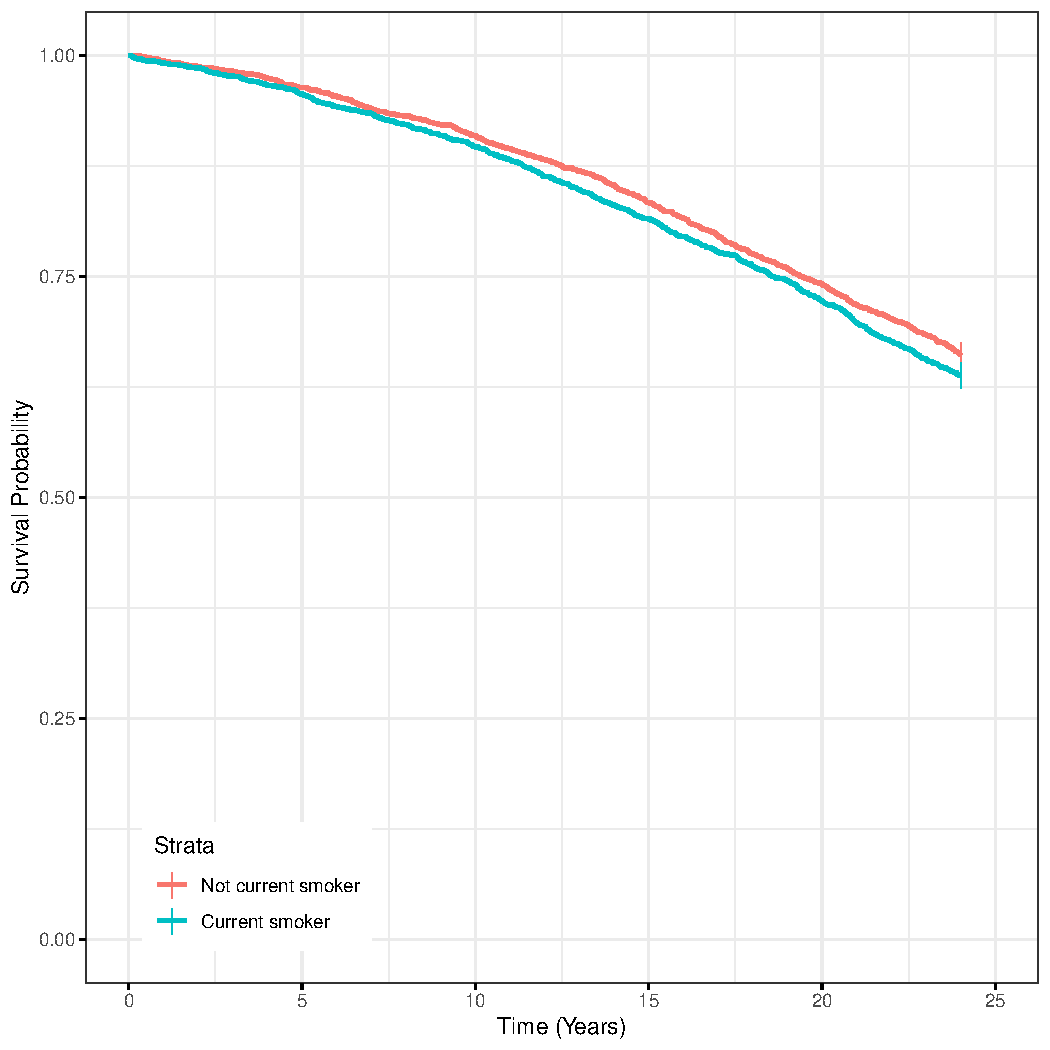
\includegraphics[width=\maxwidth]{figure/unnamed-chunk-15-1} 

\end{knitrout}


\pagebreak

\section*{Question 2}

\ifdraft

\textbf{Referring to the code from lecture}, are you able to calculate the overall median survival time in this case? If so, provide an estimate of this quantity, if not, describe why and provide an estimate of a percentile of survival time (of your choice). Interpret the quantity that you estimated. \textbf{(20 points)}

\vspace{2mm}



\fi

We cannot calculate the overall median survival time in this case because less than half of this sample had the event (death) by the end of the study.  (This dataset has no censored observations except for those right-censored at the end of the study, so the the number of participants observed to have died in this dataset equals the number who did actually die during the study period.)  In other words, over half of the observations are right-censored, and thus the true median survival time is somewhere in that majority of unobserved full survival times and unknown to us.  As over 25\% of the cohort did die over the course of the study, however, we can estimate the \textbf{25th percentile of survival time}, the first time point at which at least 25\% of the cohort had died and 75\% or less of the cohort remained alive, which was \textbf{19.09} years.  

\vspace{2mm}

(For another dataset containing censored observations throughout the study period instead of only at the end, a more accurate wording of the above might be "the first time point at which the probability of being dead in this cohort is estimated to be at least 25\%.  Both of those interpretations assume that all participants start counting follow-up time at the same time, whether in real or statistical time, which appears true for this dataset since all study entry times are 0.)

\vspace{2mm}

In other words, in this specific cohort with no censored observations until the end of the study and identical times of entry among all partiicpants, that last person who needed to die to bring the total percentage of the cohort dead to or above 25\% did so 19.09 years after the start of the study.

\vspace{2mm}

(The 25th percentile of survival time among current nonsmokers was 19.44 years, and the 25th percentile of survival time among current smokers was 18.61 years.  In other words, among members of the cohort who were nonsmokers at the beginning of the study, the first time at which at least 25\% of them had died was 19.44 years after the start of the study.  Similarly, the first time at which at least 25\% of the members of the cohort who were smokers at the beginning of the study had died was 18.61 years after the start of the study.)








\pagebreak

\section*{Question 3}

\ifdraft

Answer the following questions about the log-rank test: \textbf{(10 points total)}
  \begin{enumerate}
    \item Describe the specific null and alternative hypotheses that the log-rank test is considering here.
    \item What do you conclude from this test (use 5\% significance criteria)? List a limitation of the inference that you obtain from the log-rank test.
  \end{enumerate}

\fi

\subsection*{1}

The null hypothesis for the log-rank test here is that the survival curve for the smokers is equivalent to that for the nonsmokers.  More specifically, the null hypothesis is that the probability of survival for a nonsmoker is the same as the probability of survival for a smoker at all times during the study period, or formally:

$$ H_0: S_1(t) = S_2(t) \: \forall(t) $$

where $S_k(t)$ is the survival probability for a member of group $k$ at time $t$.  (Here, $k=1$ designates the nonsmoking group and $k=2$ designates the smoking group.)

\vspace{2mm}

The alternative hypothesis is that the survival curve for at least one group is different than the others at some time during the study period, or, formally:

$$ \exists (t) \: S_1(t) \neq S_2(t) $$

\subsection*{2}





\pagebreak

\section*{Question 4}

\ifdraft

Answer the following questions about the Cox models estimated above: \textbf{(20 points total)}
  \begin{enumerate}
    \item Why do we use specialized methods for survival analysis (instead of linear or logistic regression, for example)? (Hint: See readings from Vittinghoff et al. 2012 text.)
    \item What are the advantages of the Cox model over other survival analysis methods? What is a potential disadvantage of the Cox model?
    \item What assumptions, if any, does the standard \textbf{Cox} proportional hazards model make?
    \item Compare the test of the smoking-mortality association between the log-rank test and the likelihood ratio test from the \ul{unadjusted} Cox proportional hazards model. What do you observe? Between these two analytic approaches, which one would you prefer, and why?
  \end{enumerate}

\fi

\pagebreak

\section*{Question 5}

\ifdraft

Write the equation for the log-hazard function for the \textit{adjusted} model you estimated. \textbf{Clearly define all functions, terms (covariates), and parameters in the model. (20 points)}

\fi

\pagebreak

\section*{Question 6}

\ifdraft

Complete the following table. How would you interpret the parameter estimate that compares smokers to non-smokers in the \textbf{adjusted model}? What measure of association common in epidemiologic research does this correspond to? \textbf{(10 points)}

\fi





% latex table generated in R 3.6.1 by xtable 1.8-4 package
% Sun Nov 24 00:24:01 2019
\begin{table}[H]
\centering
\parbox{10cm}{\caption{Crude and adjusted hazard ratio (HR) estimates of the association between baseline smoking status and mortality. Framingham Cohort Study. 1948-1972, Framingham, MA.}} 
\begin{tabular}{lllll}
  \hline
Smoker & Events & Follow-Up Time (years) & Crude HR (95\% CI) & Adjusted HR (95\% CI) \\ 
  \hline
No &  &  &  &  \\ 
  Yes &  &  &  &  \\ 
   \hline
\end{tabular}
\end{table}

  
\pagebreak

\section*{Question 7}

\ifdraft

Based on the model that included covariate-by-time interactions, is there evidence for a violation of the proportional hazards assumption in any of the variables? Indicate how you arrived at your conclusion. \ul{In 1-2 sentences} describe in general how you would account for any violations in the proportional hazards assumption (ignoring whether or not there were significant differences here). \textbf{(10 points)}

\fi

\end{document}
